% This is a UHH LaTeX thesis template (German) that is built on the template
% of the UHH informatics department and the template of the Reed
% College LaTeX thesis (from the thesisdown R package).

% -------------------------------
% --- PREAMBLE ---
% -------------------------------
\documentclass[a4paper,12pt]{article}


% Coding, Language, Patches {{{
\usepackage[T1]{fontenc}    		% for coding output; allows for umlaut, accents und
                            				% correct hyphenation
\usepackage[utf8]{inputenc} 		% allows for direct input of special characters;
\usepackage[ngerman, english]{babel}
\usepackage{microtype}     		% optimal margin and scale setting
\usepackage[autostyle]{csquotes}  	% correct quotation marks in bibliograpy
\usepackage{scrhack}        		% avoids warnings with older packages
\usepackage[newcommands]{ragged2e}  % improves \ragged...commands
\PassOptionsToPackage{hyphens}{url}   % for URL line breaks in footmarks and bibliography
% }}}

% Fonts {{{
\usepackage{mathptmx}       		% use Times as default text font; modifies the default serif and math fonts
\usepackage[scaled=.92]{helvet} 	% modifies the sans serif font
\usepackage{courier}        			% modifies the monospace font
\usepackage{sectsty}        			% the alternative with {titlesec} did not work
							% make headers same style as in scrreprt document class:
%\sectionfont{\sffamily\bfseries}
%\subsectionfont{\sffamily\bfseries}
\linespread{1.25}               			% make line hight equivalent to 1.5 in MS Word
% }}}

% Document and text settings {{{
\usepackage[
    a4paper,
    margin=2.5cm,
    marginparwidth=2.0cm,
    footskip=1.0cm
    ]{geometry}
\clubpenalty=10000          			% avoids so-called 'clubs': single lines at beginning of paragraph
\widowpenalty=10000        	 	% avoids so-called 'widos': single lines at end of paragraph
\displaywidowpenalty=10000
\usepackage{ifdraft}        			% enables \ifoptionfinal{true}{false}
\pagestyle{plain}           			% no headlines
\setlength{\emergencystretch}{3em} 	% prevent overfull lines
% }}}

% Table packages {{{
\usepackage{booktabs}			% for publication quality tables in LaTeX
\usepackage{tabularx} 			% defines an environment tabularx, an extension of tabular
\usepackage{longtable}    			% handles multipage tables
\usepackage{multirow}       		% creates tabular cells spanning multiple rows
\usepackage{multicol}       			% creates tabular cells spanning multiple columns
 \usepackage{array}					% extends the array and tabular environments
% }}}

% % Other packages {{{
\usepackage{amsmath,amssymb,amsthm}    	% typical maths resource packages
\usepackage{calc}						% for simple arithmetic in LaTeX commands
\usepackage{textcomp}                           		% for single quotes
\usepackage[bf]{caption}
\usepackage[bottom, flushmargin]{footmisc}      % for footnotes
\usepackage{footnotebackref}
\usepackage{tikz}						% tool to create graphic elements in LaTeX
% }}}

% URLs {{{
\usepackage[hyphens]{url}
\urlstyle{same} 					% disable monospaced font for URLs
% }}}

% Define citation style {{{
\usepackage{natbib}       			% literature reference style
  \bibliographystyle{}
  \bibliography{bib/references.bib}
% }}}

% ToC {{{
\setcounter{secnumdepth}{5}
\setcounter{tocdepth}{5}
% }}}

  \usepackage[parfill]{parskip}


% Graphics {{{
\usepackage{graphicx}            		% packages to allow inclusion of graphics
\makeatletter
\def\maxwidth{\ifdim\Gin@nat@width>\linewidth\linewidth\else\Gin@nat@width\fi}
\def\maxheight{\ifdim\Gin@nat@height>\textheight\textheight\else\Gin@nat@height\fi}
\makeatother

% Define position of graphics
\usepackage{float}
\floatplacement{figure}{H}
\floatplacement{table}{H}			% to change the default alignment of an image
\usepackage[export]{adjustbox}
% }}}


% Colors {{{
\usepackage{xcolor}				% extends LATEX's color facilities
\usepackage{colortbl}			% to add colour to LaTeX tables

% Define colors for hyperlinks:
\definecolor{linkcol}{HTML}{014979} 		% darkblue
\definecolor{filecol}{HTML}{b70000} 		% darkred
\definecolor{urlcol}{HTML}{b70000} 		% darkred
\definecolor{citecol}{HTML}{4c4c4c} 		% darkgray


% Hypersetup {{{
\hypersetup{
colorlinks=true,
linkcolor=linkcol,
filecolor=filecol,
urlcolor=urlcol,
citecolor=citecol,
linktocpage=true,
pdfpagemode=UseOutlines,
}
% }}}

% Cross-referencing {{{
% Use ref for internal links
\usepackage{hyperref}     			% to handle cross-referencing commands in LaTeX
\renewcommand{\hyperref}[2][???]{\autoref{#1}}
\def\chapterautorefname{Chapter}
\def\sectionautorefname{Section}
\def\subsectionautorefname{Subsection}
% }}}


% Define tightlist to work with newer versions of pandoc
\providecommand{\tightlist}{%
  \setlength{\itemsep}{0pt}\setlength{\parskip}{0pt}}

% Save thesis parameters for later
\newcommand{\thesistype}{Bachelorarbeit / Masterarbeit}
\newcommand{\thesisauthor}{Mandy Mustermann}
\newcommand{\thesisdate}{}


% Syntax highlighting
  \usepackage{color}
  \usepackage{fancyvrb}
  \newcommand{\VerbBar}{|}
  \newcommand{\VERB}{\Verb[commandchars=\\\{\}]}
  \DefineVerbatimEnvironment{Highlighting}{Verbatim}{commandchars=\\\{\}}
  % Add ',fontsize=\small' for more characters per line
  \usepackage{framed}
  \definecolor{shadecolor}{RGB}{248,248,248}
  \newenvironment{Shaded}{\begin{snugshade}}{\end{snugshade}}
  \newcommand{\AlertTok}[1]{\textcolor[rgb]{0.94,0.16,0.16}{#1}}
  \newcommand{\AnnotationTok}[1]{\textcolor[rgb]{0.56,0.35,0.01}{\textbf{\textit{#1}}}}
  \newcommand{\AttributeTok}[1]{\textcolor[rgb]{0.77,0.63,0.00}{#1}}
  \newcommand{\BaseNTok}[1]{\textcolor[rgb]{0.00,0.00,0.81}{#1}}
  \newcommand{\BuiltInTok}[1]{#1}
  \newcommand{\CharTok}[1]{\textcolor[rgb]{0.31,0.60,0.02}{#1}}
  \newcommand{\CommentTok}[1]{\textcolor[rgb]{0.56,0.35,0.01}{\textit{#1}}}
  \newcommand{\CommentVarTok}[1]{\textcolor[rgb]{0.56,0.35,0.01}{\textbf{\textit{#1}}}}
  \newcommand{\ConstantTok}[1]{\textcolor[rgb]{0.00,0.00,0.00}{#1}}
  \newcommand{\ControlFlowTok}[1]{\textcolor[rgb]{0.13,0.29,0.53}{\textbf{#1}}}
  \newcommand{\DataTypeTok}[1]{\textcolor[rgb]{0.13,0.29,0.53}{#1}}
  \newcommand{\DecValTok}[1]{\textcolor[rgb]{0.00,0.00,0.81}{#1}}
  \newcommand{\DocumentationTok}[1]{\textcolor[rgb]{0.56,0.35,0.01}{\textbf{\textit{#1}}}}
  \newcommand{\ErrorTok}[1]{\textcolor[rgb]{0.64,0.00,0.00}{\textbf{#1}}}
  \newcommand{\ExtensionTok}[1]{#1}
  \newcommand{\FloatTok}[1]{\textcolor[rgb]{0.00,0.00,0.81}{#1}}
  \newcommand{\FunctionTok}[1]{\textcolor[rgb]{0.00,0.00,0.00}{#1}}
  \newcommand{\ImportTok}[1]{#1}
  \newcommand{\InformationTok}[1]{\textcolor[rgb]{0.56,0.35,0.01}{\textbf{\textit{#1}}}}
  \newcommand{\KeywordTok}[1]{\textcolor[rgb]{0.13,0.29,0.53}{\textbf{#1}}}
  \newcommand{\NormalTok}[1]{#1}
  \newcommand{\OperatorTok}[1]{\textcolor[rgb]{0.81,0.36,0.00}{\textbf{#1}}}
  \newcommand{\OtherTok}[1]{\textcolor[rgb]{0.56,0.35,0.01}{#1}}
  \newcommand{\PreprocessorTok}[1]{\textcolor[rgb]{0.56,0.35,0.01}{\textit{#1}}}
  \newcommand{\RegionMarkerTok}[1]{#1}
  \newcommand{\SpecialCharTok}[1]{\textcolor[rgb]{0.00,0.00,0.00}{#1}}
  \newcommand{\SpecialStringTok}[1]{\textcolor[rgb]{0.31,0.60,0.02}{#1}}
  \newcommand{\StringTok}[1]{\textcolor[rgb]{0.31,0.60,0.02}{#1}}
  \newcommand{\VariableTok}[1]{\textcolor[rgb]{0.00,0.00,0.00}{#1}}
  \newcommand{\VerbatimStringTok}[1]{\textcolor[rgb]{0.31,0.60,0.02}{#1}}
  \newcommand{\WarningTok}[1]{\textcolor[rgb]{0.56,0.35,0.01}{\textbf{\textit{#1}}}}

% Additional LaTeX parameters added in the YAML header of index.Rmd



\begin{document}

% -------------------------------
% --- frontmatter: Title page ---
% -------------------------------
\thispagestyle{empty}
\begin{titlepage}


\includegraphics[width=6.8cm]{images/uhh_logo.png}
\hspace{2cm}

\includegraphics[width=7cm]{images/min_logo.png}
\begin{center}\Large
  \vfill
	Bachelorarbeit / Masterarbeit
	\vfill
	\makeatletter
	{\LARGE\textsf{\textbf{Titel der Abschlussarbeit}}\par}
	\makeatother
	\vfill
  vorgelegt von \\\vspace{0.5cm}
  \par\bigskip
	\makeatletter
  \textbf{Mandy Mustermann} \\
  \makeatother
  geb. am 31. Januar 1970 \\
  Matrikulationsnummer: 1234567 \\
  Studiengang: Biologie \\
  \vfill
	\makeatletter
	eingereicht am 1. April 2000
	\makeatother
	\vfill
  1. Gutachter: Prof.~Dr. \\
  2. Gutachter: Prof.~Dr. \\

\end{center}
\end{titlepage}

% -----------------------------
% --- frontmatter: Abstract ---
% -----------------------------
\newpage
\hypertarget{abstract}{%
\section*{Abstract}\label{abstract}}
\addcontentsline{toc}{section}{Abstract}

Auf etwa einer halben, maximal einer Seite sollten die wichtigsten Inhalte, Erkenntnisse, Neuerungen bzw. Ergebnisse der Arbeit beschrieben werden.
Durch eine solche Zusammenfassung, im Engl. auch \emph{Abstract} genannt, am Anfang der Arbeit wird die Arbeit deutlich aufgewertet. Hier sollte vermittelt werden, warum der Leser die Arbeit lesen sollte.

Die Englische Zusammenfassung erfolgt zuerst.
\pagestyle{plain}
\pagenumbering{roman}   		% define page number in roman style
\setcounter{page}{1}    		% start page numbering

% ------------------------------------
% --- frontmatter: Zusammenfassung ---
% ------------------------------------
\newpage
\hypertarget{zusammenfassung}{%
\section*{Zusammenfassung}\label{zusammenfassung}}
\addcontentsline{toc}{section}{Zusammenfassung}

Die Deutsche Zusammenfassung sollte eine direkte Übersetzung des Englischen \emph{Abstract} sein und sich inhaltlich nicht unterscheiden.

% -----------------------------
% --- frontmatter: Contents ---
% -----------------------------
\newpage
\renewcommand{\contentsname}{Inhaltsverzeichnis}
\tableofcontents
\clearpage

% ----------------------------------------------------------
% --- frontmatter: List of Abbreviations (not mandatory) ---
% ----------------------------------------------------------
\newpage
\hypertarget{abkurzungsverzeichnis}{%
\section*{Abkürzungsverzeichnis}\label{abkurzungsverzeichnis}}
\addcontentsline{toc}{section}{Abkürzungsverzeichnis}

Sie können zur Auflistung von Abkürzungen eine Tabelle mittels R Markdown oder \LaTeX Syntax erstellen. Bei der \LaTeX Variante ist allerdings der Vorteil, dass die Tabelle keine automatische Nummer erhält und daher nicht im Tabellenverzeichnis erscheint. Auch startet die nächste Tabelle im Haupttext mit der Nummer 2!

\vspace{1cm}
\begin{tabular}{*2{l}}
    ATP  &  Adenosintriphosphat   \\ 
    CoA  &  Coenzym A  \\
    DNA  &  Desoxyribonukleinsäure \\         
    mtDNA  &  Mitochondriale DNA \\
\end{tabular}
% ----------------------------------------------------
% --- frontmatter: List of Figures (not mandatory) ---
% ----------------------------------------------------
\newpage
\listoffigures
\addcontentsline{toc}{section}{Abbildungsverzeichnis}

% ---------------------------------------------------
% --- frontmatter: List of Tables (not mandatory) ---
% ---------------------------------------------------
\newpage
\listoftables
\addcontentsline{toc}{section}{Tabellenverzeichnis}

% -------------------------------
% --- main body of the thesis ---
% -------------------------------
\newpage
\pagestyle{plain}
\setcounter{page}{1}    		% start page numbering anew
\pagenumbering{arabic}  		% page numbers in arabic style

\hypertarget{einstellungen-im-yaml-header}{%
\section*{Einstellungen im YAML Header}\label{einstellungen-im-yaml-header}}
\addcontentsline{toc}{section}{Einstellungen im YAML Header}

Im Folgenden gibt es einige Hinweise zu den Einstellungen des Dokumentes, die in den sog. YAML (\emph{YAML Ain't Markup Language}) Kopfzeilen vorgenommen werden können. Dieser Abschnitt kann später gelöscht werden. Im übrigen kann die Nummerierung des Abschnitts bzw. Kapitels mit einem \texttt{\{-\}} hinter der Überschrift rausgenommen werden (dies wird hier gemacht wie auch im Abstract, der Zusammenfassung, den Verzeichnissen, der Danksagung und eidesstattlichen Versicherung).
\begin{itemize}
\tightlist
\item
  Diese .Rmd Datei ist die eigentliche R Markdown Datei, die \enquote{geknitted} wird, um die gesamte PDF-Datei zu erstellen. Wichtig ist, dass sie unter dem Namen \texttt{index.Rmd} abgespeichert wird. Alle anderen .Rmd Dateien werden \textbf{NICHT} \enquote{geknitted}!!!
\item
  Im obigen YAML Kopfzeilenbereich sind bereits alle wichtigen YAML Einstellungen sowie Blindtexte gesetzt, die noch für das Titelblatt ausgetauscht werden müssen. Hinweis: wenn es Probleme beim \enquote{knitten} gibt, könnten Leerzeichen die Ursache sein.
\item
  Die Liste an Referenzen kann entweder in die oben angegebene Datei \enquote{bib/references.bib} eingefügt werden, oder der Pfad zur einer anderen Datei wird aufgeführt. Der Referenzstil wird mit der Datei .csl festgelegt, kann aber gegen eine andere ausgetauscht werden. Der aktuelle Stil orientiert sich am \href{https://uk.sagepub.com/sites/default/files/sage_harvard_reference_style_0.pdf}{SAGE Harvard} Referenzstil. Weitere Informationen sind auch unter \protect\hyperlink{zitate-und-literaturverzeichnis}{Zitate und Literaturverzeichnis} zu finden.
\item
  Hyperlinks: die Standardfarben für interne Querverweise (inkl. Inhaltsverzeichnis), externe Querverweise, Zitatverweise und verlinkte URLs können angepasst werden, indem die YAML Parameter \texttt{linkcolor}, \texttt{filecolor}, \texttt{citecolor} bzw. \texttt{urlcolor} mit entsprechendem LaTeX Farbnamen gelistet werden, z.B. \texttt{linkcolor:\ red}.
\item
  Die Funktion zur Umwandlung vom R Markdown zum PDF/LaTeX ist \texttt{pdf\_thesis\_dt} und sollte immer relativ am Ende des YAML Kopfbereich stehen:
\end{itemize}
\begin{verbatim}
output:
  UHHformats::pdf_thesis_dt:
    toc: true
    toc_depth: 5
    highlight: default
    citation_package: natbib
\end{verbatim}
Die Standardeinstellungen von \texttt{toc}, \texttt{toc\_depth}, \texttt{highlight} und \texttt{citation\_package} sind hier angezeigt, müssen aber nicht im YAML header extra gesetzt werden, außer diese sollen explizit geändert werden. Weitere Optionen, die hier gelistet werden können, können der \texttt{bookdown::pdf\_book} Funktion entnommen werden, auf der \texttt{UHHformats::pdf\_thesis\_dt} basiert.

Die Texte der Abschnitte \emph{Abstract}, \emph{Zusammenfassung} und das \emph{Abkürzungsverzeichnis} werden in separaten Dateien im Ordner \texttt{prelim/} aufgeführt:
\begin{itemize}
\tightlist
\item
  \texttt{00-abstract.Rmd}
\item
  \texttt{00-zusammenfassung.Rmd}
\item
  \texttt{00-abkuerzungen.Rmd}
\end{itemize}
Alle anderen Kapitel werden in einzelnen .Rmd Dateien im Ordner \texttt{chapter/} aufgeführt:
\begin{itemize}
\tightlist
\item
  \texttt{01-einleitung.Rmd}
\item
  \texttt{02-methodik.Rmd}
\item
  \texttt{03-ergebnisse.Rmd}
\item
  \texttt{04-diskussion.Rmd}
\item
  \texttt{96-referenzen.Rmd}
\item
  \texttt{97-anhang.Rmd}
\item
  \texttt{98-danksagung.Rmd}
\item
  \texttt{99-versicherung.Rmd}
\end{itemize}
Die Reihenfolge der einzelnen Abschnitte und Kapitel wird in der Datei \texttt{\_bookdown.yml} festgelegt. Falls weitere Kapitel (im Ordner \texttt{chapter/}) hinzugefügt werden sollen, einfach die Dateinamen dieser neuen .Rmd Dateien in die \texttt{\_bookdown.yml} Datei mit auflisten.

Eine gute Hilfe ist das Onlinebuch \href{https://bookdown.org/yihui/bookdown/}{bookdown: Authoring Books and Technical Documents with R Markdown}, auf dem diese Vorlage basiert.

\hypertarget{einleitung}{%
\section{Einleitung}\label{einleitung}}

Die Bachelor- und Masterarbeit kann in deutscher oder englischer Sprache verfasst werden. Die Seitenzahl sollte dem Arbeitsaufwand der Bachelor- (12LP) bzw. Masterarbeit (30LP) insgesamt entsprechen (ggf. Rücksprache mit dem Anleiter). Die Arbeit ist in dreifacher Ausfertigung (gebunden; keine Spiralbindung) und als eine PDF Datei auf zwei CD-ROMs (flexible CD-Hülle) im Studienbüro abzugeben (rechtzeitig!)

\hypertarget{struktur-und-form-der-arbeit}{%
\subsection{Struktur und Form der Arbeit}\label{struktur-und-form-der-arbeit}}

Die wissenschaftliche Arbeit sollte sich aus folgenden Abschnitten zusammensetzen, welche bereits in dieser Vorlage eingerichtet wurden:
\begin{enumerate}
\def\labelenumi{\arabic{enumi}.}
\tightlist
\item
  \textbf{Titelblatt} {[}wird automatisch über den YAML Kopfbereich erstellt{]}
\item
  \textbf{Zusammenfassung} auf Englisch (\textbf{Abstract}) und Deutsch {[}s. Dateien im \texttt{prelim/} Ordner{]}
\item
  \textbf{Inhaltsverzeichnis} {[}wird hier automatisch erstellt{]}
\item
  \textbf{Abkürzungsverzeichnis} (optional) {[}s. Datei im \texttt{prelim/} Ordner{]}
\item
  \textbf{Tabellen}- und \textbf{Abbildungsverzeichnis} (optional) {[}wird hier automatisch erstellt wenn im YAML Kopfbereich \texttt{lot:\ true} und \texttt{lof:\ true} stehen bleibt{]}
\item
  \textbf{Einleitung} {[}s. Datei im \texttt{chapter/} Ordner{]}
\item
  \textbf{Material \& Methoden} {[}s. Datei im \texttt{chapter/} Ordner{]}
\item
  \textbf{Ergebnisse} {[}s. Datei im \texttt{chapter/} Ordner{]}
\item
  \textbf{Diskussion} {[}s. Datei im \texttt{chapter/} Ordner{]}
\item
  \textbf{Literaturverzeichnis} {[}die entsprechende .bib Datei mit den einzelnen Referenzen muss im YAML Kopfbereich angegeben werden{]}
\item
  \textbf{Anhang} (optional) {[}s. Datei im \texttt{chapter/} Ordner{]}
\item
  \textbf{Danksagung} (optional) {[}s. Datei im \texttt{chapter/} Ordner{]}
\item
  \textbf{Eidesstattliche Versicherung} (Pflicht) - Datum und Unterschrift hier nicht vergessen {[}s. Datei im \texttt{chapter/} Ordner{]}
\end{enumerate}
Grundsätzlich sollte folgendes Format eingehalten werden: Schriftgröße 12 Times New Roman, Zeilenabstand 1,5, Seitenränder jeweils 2,5cm, Oberer Rand 2,5cm unterer Rand 2,0cm. Dies ist bereits in dieser Vorlage festgelegt und muss nicht weiter angepasst werden!

\hypertarget{inhalt-der-einleitung}{%
\subsection{Inhalt der Einleitung}\label{inhalt-der-einleitung}}

Die Einleitung setzt sich aus der Problemstellung, deren Relevanz sowie Zielsetzung und Aufbau der Arbeit zusammen. Die Einleitung sollte dabei immer vom Allgemeinen ins Spezifische gehen. Es sollten in knapper Form folgende Fragen beantwortet werden:
\begin{itemize}
\tightlist
\item
  Was ist das allgemeine Thema?
\item
  Was ist die spezifische Fragestellung der Arbeit, welches Ziel wird verfolgt? Warum ist die Frage wichtig?
\item
  Wie wurde die Frage bisher in der Literatur behandelt?
\item
  Welche Hypothese wird in der vorliegenden Arbeit (statistisch) getestet?
\item
  Wie ist der folgende Text gegliedert? (Argumentationskette, Teilprobleme)
\end{itemize}
\hypertarget{literatur}{%
\subsection{Literatur}\label{literatur}}

Das Heraussuchen und Verwenden relevanter akademischer Literatur ist ein wichtiger Bestandteil von Abschlussarbeiten.

\hypertarget{literaturrecherche}{%
\subsubsection{Literaturrecherche}\label{literaturrecherche}}

Bei der Literatursuche empfiehlt es sich mit der vorgegebenen Einstiegsliteratur und den darin zitierten Quellen zu beginnen. Viele Titel lassen sich bequem über \href{https://apps.webofknowledge.com/WOS_GeneralSearch_input.do?product=WOS\&search_mode=GeneralSearch\&SID=E4BQAzXmvUw7kPeUIBE\&preferencesSaved=}{Web of Science} oder \href{https://scholar.google.de/}{Google Scholar} suchen und finden. Dabei kann die Anzahl an Zitierungen einen brauch- baren Hinweis auf die Relevanz eines bestimmten Titels liefern. Die Web of Science Datenbank kann allerdings nur von der Uni aus aufgerufen werden oder von zuhause über einen \href{https://www.rrz.uni-hamburg.de/services/netz/vpn.html}{VPN} client.

Wichtige Literaturquellen sind
\begin{enumerate}
\def\labelenumi{\arabic{enumi}.}
\tightlist
\item
  Fachbücher, Standards
\item
  Wiss. Zeitschriftenartikel
\item
  Konferenzbeiträge
\item
  Universitäre Abschlussarbeiten
\item
  Technische Berichte, graue Literatur
\item
  Online-Material, Ausarbeitungen
\end{enumerate}
Weitere wichtige Literaturdatenbanken im Fachbereich Biologie sind neben Web of Science und Google Scholar u.a. noch
\begin{itemize}
\tightlist
\item
  die \href{https://www.sub.uni-hamburg.de/recherche/elektronische-zeitschriftenbibliothek.html}{Elektronische Zeitschriftenbibliothek der Universität Hamburg} (EZB)
\item
  die \href{https://www.biologie.uni-hamburg.de/service/bibliotheken/bibliothek-fachbereichsbibliothek/digibib.html}{Digitale Bibliothek} der Fachbereichsbibliothek der UHH Biologie
\item
  die \href{http://www.vifabio.de/}{virtuelle Fachbibliothek Biologie} (vifabio) der \href{https://www.ub.uni-frankfurt.de/}{Universitätsbibliothek Johann Christian Senckenberg}
\item
  die Kataloge und Datenbanken die in der vifabio gelistet sind: \url{http://www.vifabio.de/howto/info/icatalogs.html}
\item
  \href{https://www.sciencedirect.com}{ScienceDirect}
\end{itemize}
\hypertarget{zitate-und-literaturverzeichnis}{%
\subsubsection{Zitate und Literaturverzeichnis}\label{zitate-und-literaturverzeichnis}}

Für alle wissenschaftlichen Arbeiten gilt: Wo immer möglich, sollte auf andere relevante Veröffentlichungen verwiesen werden, anstatt deren Inhalt noch einmal wiederzugeben. Für alle Aussagen und Darstellungen, die aus Veröffentlichungen stammen, sind Quellenangaben zu machen. Bei Inhalten aus fremden Quellen, die paraphrasiert oder wörtlich übernommen werden, ist die Quellenangabe an der Textstelle zu machen. Es genügt nicht, die Quelle ins Literaturverzeichnis aufzunehmen. Wörtliche Übernahmen von längeren Wortgruppen und ganzen Sätzen sind in Anführungszeichen zu setzen.

Zur Erstellung von Literaturangaben und -verzeichnissen wird hier das Programm BibTeX verwendet. Der Vorteil von BibTeX bzw. einer Literaturdatenbank ist, dass alle Zitate und Quellenverweise im gesamten Dokument automatisch herausgesucht und über eine Literaturdatenbank den entsprechenden Werken zugeordnet werden. Die .bib Datei, auf die im YAML Kopfbereich verwiesen wird, stellt hierbei die Literaturdatenbank dar. Diese Datei ist eine sog. plain-text Datei, welche bibliographische Einträge in folgender Form enthält:
\begin{Shaded}
\begin{Highlighting}[]
\OperatorTok{@}\NormalTok{article\{May1976,}
\NormalTok{   author =}\StringTok{ }\NormalTok{\{May, R. M.\},}
\NormalTok{   title =}\StringTok{ }\NormalTok{\{Simple mathematical models with very }
\NormalTok{     complicated dynamics\},}
\NormalTok{   journal =}\StringTok{ }\NormalTok{\{Nature\},}
\NormalTok{   volume =}\StringTok{ }\NormalTok{\{}\DecValTok{261}\NormalTok{\},}
\NormalTok{   number =}\StringTok{ }\NormalTok{\{}\DecValTok{5560}\NormalTok{\},}
\NormalTok{   pages =}\StringTok{ }\NormalTok{\{}\DecValTok{459-467}\NormalTok{\},}
\NormalTok{   ISSN =}\StringTok{ }\NormalTok{\{}\DecValTok{0028-0836}\NormalTok{\},}
\NormalTok{   DOI =}\StringTok{ }\NormalTok{\{}\FloatTok{10.1038}\OperatorTok{/}\NormalTok{261459a0\},}
\NormalTok{   url =}\StringTok{ }\NormalTok{\{}\OperatorTok{<}\NormalTok{Go to ISI}\OperatorTok{>}\ErrorTok{://}\NormalTok{WOS}\OperatorTok{:}\NormalTok{A1976BT72500018\},}
\NormalTok{   year =}\StringTok{ }\NormalTok{\{}\DecValTok{1976}\NormalTok{\},}
\NormalTok{   type =}\StringTok{ }\NormalTok{\{Journal Article\}}
\NormalTok{\}}
\end{Highlighting}
\end{Shaded}
Ein einzelner Eintrag fängt immer mit \texttt{@type\{} an, wobei der Typ ein \texttt{article}, \texttt{book}, \texttt{manual}, \texttt{techreport}, \texttt{inproceedings}, \texttt{phdthesis} oder \texttt{misc} (bei z.B. Multimedia Typen, Computerprogramm) sein kann. Mehr Informationen zu den möglichen Typen sowie zu den einzelnen Feldern wie \texttt{author}, \texttt{title}, etc. gibt es unter \url{https://de.wikipedia.org/wiki/BibTeX}. Anschl. kommt nach der geschweiften Klammer der Referenzschlüssel bzw. der ‚citation key`. Um einen dieser Einträge bzw. Referenzen zu zitieren wird das @ Zeichen mit dem Schlüssel kombiniert:
\begin{itemize}
\tightlist
\item
  \texttt{@May1976} --\textgreater{} wird zu May (\protect\hyperlink{ref-May1976}{1976})
\item
  \texttt{{[}@May1976{]}} --\textgreater{} wird zu (May, \protect\hyperlink{ref-May1976}{1976})
\end{itemize}
Bei Verwendung der eckigen Klammern erscheint also der Autorname zusammen mit der Jahreszahl in der runden Klammer.

In der R Markdown Datei würde man z.B. schreiben \enquote{\texttt{@May1976} konnte zeigen, dass einfache Populationsmodelle komplexe chaotische Dynamiken auslösen können.}, was im PDF/LaTeX Dokument dann zu \enquote{May (\protect\hyperlink{ref-May1976}{1976}) konnte zeigen \ldots{}} übersetzt wird. Alle Referenzen erhalten automatischen einen Hypertext-Link zum Literaturverzeichnis. Falls dies nicht erwünscht ist, muss im YAML Kopfbereich \texttt{link-citation:\ false} angegeben werden.

Mehreren zitierte Quellen werden mit einem Semikolon getrennt, z.B. (Kamm, \protect\hyperlink{ref-kamm2000}{2000}; May, \protect\hyperlink{ref-May1976}{1976}; Post and Forchhammer, \protect\hyperlink{ref-RN410}{2002})

Die Formatierung des Literaturverzeichnis ist variabel. Der im Dokument eingestellte BibTeX-Stil (engl. style) bestimmt, welche Angaben in welcher Formatierung dargestellt werden. Der Stil wird im YAML Kopfbereich über die .csl Datei festgelegt. CSL steht für \emph{Citation Style Language} und ist eine XML-Sprache zur Beschreibung von Formaten für bibliografische Angaben und Referenzstile. Statt dem aktuellen \href{https://uk.sagepub.com/sites/default/files/sage_harvard_reference_style_0.pdf}{SAGE Harvard} Stils kann jeder andere Stil verwendet werden indem auf eine andere .csl Datei verwiesen wird. Es gibt auf GitHub eine sog. \enquote{repository}, welche eine Vielzahl von .csl Datei für die entsprechenden Stile bereit stellt: \url{https://github.com/citation-style-language/styles}.

Um das Organisieren, Austauschen und Zitieren von wissenschaftlichen Artikeln und PDF-Dokumenten in dieser wie auch weiteren Arbeiten zu erleichtern, empfiehlt es sich ein Literaturverwaltungsprogramm oder Referenzmanager, wie z.B. \href{https://www.mendeley.com/?interaction_required=true}{Mendeley} oder \href{https://www.zotero.org/}{Zotero}, von Anfang an zu verwenden. Damit lassen sich auch .bib Dateien für einzelne Arbeiten erstellen.

Ein sehr nützliches R Studio add-in mit dem man ganz leicht Quellen über eine GUI (graphische Oberfläche) einfügen kann ist das Paket {[}citr{]}((\url{https://github.com/crsh/citr}). Wenn man Zotero als Referenzmanager verwendet, kann \texttt{citr} auch direkt auf dessen Datenbank zugreifen.

\newpage

\hypertarget{material-und-methodik}{%
\section{Material und Methodik}\label{material-und-methodik}}

Was genau in diesem Kapitel aufgeführt wird, hängt sehr von der Art der Abschlussarbeit ab, ob es sich um ein Laborexperiment, eine Feldstudie oder eine theoretische bzw. Modellierungsarbeit handelt. Bei Feldstudien ergeben sich typischerweise folgende Abschnitte:
\begin{itemize}
\tightlist
\item
  Untersuchungsgebiet
\item
  Datenerhebung/Sampling Design
\item
  Statistische Analyse mit Angabe der entsprechenden Computerprogramme\footnote{wie \href{https://cran.r-project.org/}{R} - so macht man übrigens eine Fußnote}
\end{itemize}
\hypertarget{untersuchungsgebiet}{%
\subsection{Untersuchungsgebiet}\label{untersuchungsgebiet}}

Externe Grafiken, wie z.B. Karten des Untersuchungsgebietes (siehe Abbildung \ref{fig:location}, lassen sich über die Funktion \texttt{knitr::include\_graphics()} einbetten:
\begin{figure}

{\centering 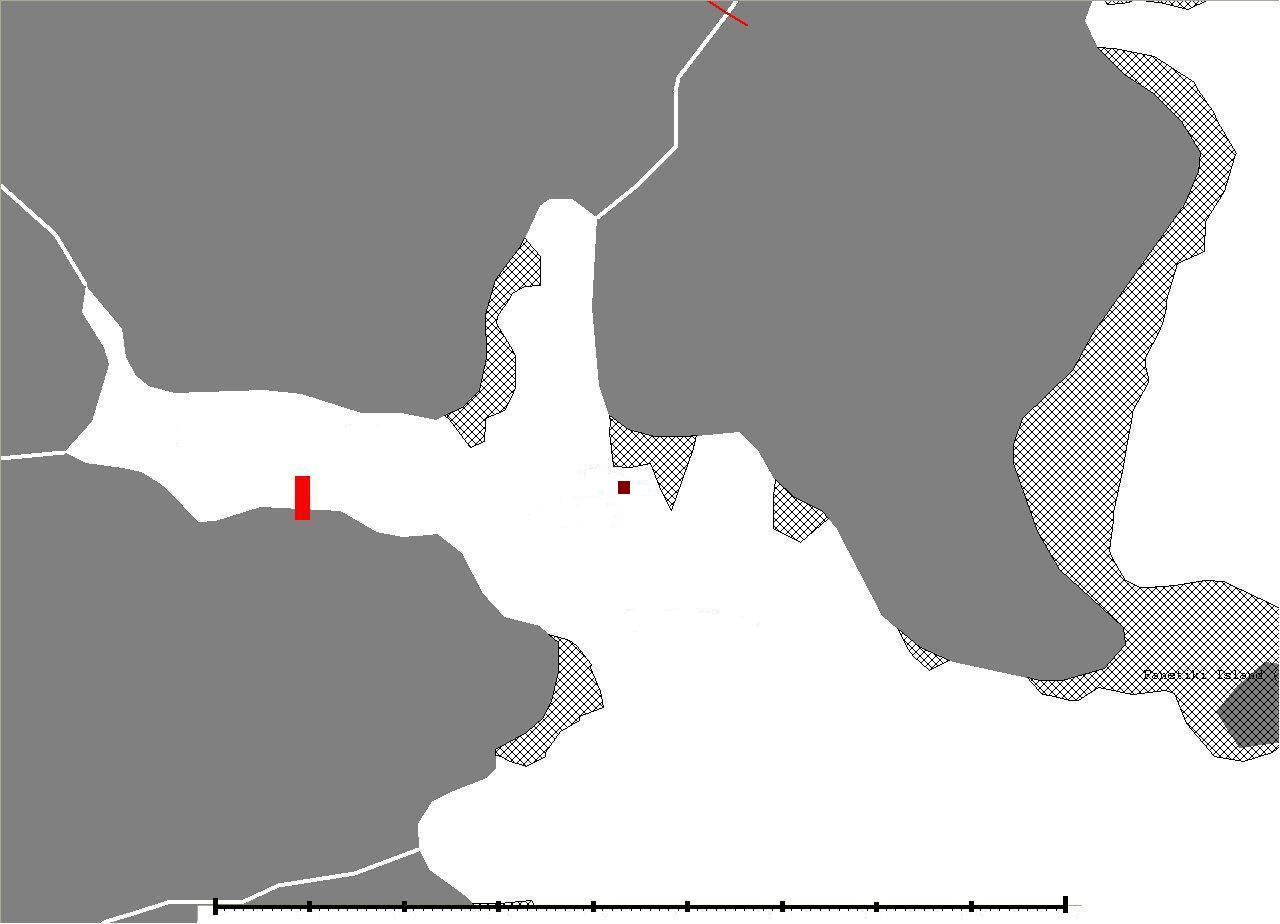
\includegraphics[width=0.5\linewidth]{images/sampling_site} 

}

\caption{Lage des Untersuchungsstandort....}\label{fig:location}
\end{figure}
\hypertarget{querverweise}{%
\subsection{Querverweise}\label{querverweise}}

Indem man dem Codeschnipsel (im Englischen \enquote{code chunk}) einen Namen (in obigen Beispiel \emph{location}) \textbf{und} eine Bildlegende (=fig.cap) gibt, lassen sich Querverweise zu Abbildungen (externe Bilddateien und R Plots) mit \texttt{\textbackslash{}@ref(fig:\textless{}label\textgreater{})} generieren. \texttt{\textless{}label\textgreater{}} ist hierbei der Name des Codeschnipsels und \texttt{fig:} gibt an, dass es sich um eine Abbildung handelt. Wichtig ist, dass die Namen der Codeschnipsel \textbf{keinen Unterstrich} enthalten. Stattdessen können Bindestriche verwendet werden.

Querverweise zu anderen Kapiteln und Unterkapiteln erfolgen ganz einfach über eckige Klammern um den Kapitelnamen, z.B. ein link zur \protect\hyperlink{diskussion}{Diskussion} via \texttt{{[}Diskussion{]}}.

Tabellen werden ähnlich verlinkt wie Abbildungen nur dass statt \texttt{fig:} ein \texttt{tab:} angegeben wird. Dies ist z.B. ein Querverweis zu Tabelle \ref{tab:kable1} im \protect\hyperlink{ergebnisse}{Ergebnisse} Kapitel.

Tabellen müssen ähnlich wie Abbildungen ein Label und eine Bildüberschrift haben, um Querverweise erstellen zu können. Allerdings enthalten die Querverweise ein \texttt{tab:} in \texttt{\textbackslash{}@ref(tab:\textless{}name\textgreater{})}) anstelle von \texttt{fig:}. Die Bildüberschrift bei Tabellen die mit R erzeugt werden, können nicht wie bei Abbildungen im Codeschnipsel selbst vergeben werden sondern in der R Funktion selbst (für Beispiele siehe das Kapitel \protect\hyperlink{ergebnisse}{Ergebnisse}.

Dies ist ein Beispiel für einen Querverweis zu Tabelle \ref{tab:kable1} im Kapitel \protect\hyperlink{die-pakete-knitr-und-kableextra}{Die Pakete \texttt{knitr} und \texttt{kableExtra}}.

\textbf{Wichtiger Hinweis}: Labels von Tabellen die direkt in Markdown geschrieben werden in der \LaTeX Notation erzeugt. Es müssen daher auch die Querverweise in \LaTeX gemacht werden. Ein Beispiel dazu wird in \protect\hyperlink{r-markdown-tabellen}{R Markdown Tabellen} gezeigt.

\hypertarget{mathematische-gleichungen}{%
\subsection{Mathematische Gleichungen}\label{mathematische-gleichungen}}

Gleichungen erzeugt man in R Markdown mit dem Dollarzeichen am Anfang und Ende. Wird jeweils ein Zeichen verwendet, wir die Gleichung in den Textfluss eingebettet, will man die Gleichung in einer eigenen Zeile (mittig), muss man 2 Zeichen werden. Dies ist z.B. der sog. \textbf{inline mode} \(E = mc^2\) und dies ist der sog. \textbf{display mode}: \[E = mc^2\]

Ganz wichtig hier ist, dass sich kein Leerzeichen zwischen \texttt{\$} und Gleichung befindet!!

Alternativ kann die Gleichung direkt in \LaTeX geschrieben werden, was einem mehr Kontrolle gibt und kompliziertere Gleichungen zulässt. Gleichungen werden auch automatisch nummeriert, was für Querverweise nützlich ist (es sei denn man setzt einen Stern hinter \texttt{\{equation*\}} wie in der letzten Gleichung). Das Label für einen Querverweis wird mit \texttt{\textbackslash{}label\{eq:label\}} gesetzt, welches direkt hinter dem \texttt{\textbackslash{}begin\{equation\}} Element kommt (siehe Gleichung \eqref{eq:mean}):
\begin{equation} \label{eq:mean}
  \bar{X} = \frac{\sum_{i=1}^n X_i}{n} 
\end{equation}
Formeln und zugehörige Erläuterungen sind immer in Sätze zu integrieren, enden also entsprechend mit Komma oder Satzpunkt. Ein Beispiel wird nachfolgend dargestellt:

Die Zufallsvariable \(Y\) sei standardnormalverteilt, d.h. \(Y \sim N(0,1)\). Dann besitzt \(Y\) die Dichtefunktion
\begin{equation} \label{eq:density-norm}
  f_{Y}(y)=\varphi(y) \stackrel{\mathrm{def}}{=} \frac{1}{\sqrt{2 \pi}} \exp \left\{ -\frac{y^2}{2} \right\}, y \in \mathbb{R}.
\end{equation}
Dabei bezeichnet \(\pi\) die Kreiszahl. Die Funktion
\begin{equation*}
  F_{Y}(y) = \Phi(y) \stackrel{\mathrm{def}}{=} \int_{-\infty}^y \varphi(x) \,\mathrm{d}x, \quad y \in \mathbb{R},
\end{equation*}
ist die zu \eqref{eq:density-norm} gehörige Verteilungsfunktion.

Die Nummerierung von Gleichungen, wie bei Gleichung \eqref{eq:density-norm}, erfolgt nur, wenn auf diese im übrigen Text verwiesen wird. Insbesondere dann, wenn in der Arbeit viele Formeln vorkommen, erscheint die Verwendung von \LaTeX sinnvoller.

\hypertarget{ergebnisse}{%
\section{Ergebnisse}\label{ergebnisse}}

Der Ergebnisteil ist für den Aufbau einer empirischen Arbeit extrem wichtig und sollte eine gute Mischung aus Text, Tabellen und Abbildungen sein. Um dem Leser eine Struktur zu geben und den roten Faden nicht zu verlieren, sollten die Forschungsfragen und Hypothesen für die Einteilung und Darstellung der Ergebnisse genutzt werden.

Abbildungen und Tabellen gehören grundsätzlich zum Text, solange sie in den Fließtext eingebunden sind. Sie werden fortlaufend nummeriert, beschriftet und ggf. mit der entsprechenden Quelle versehen. Außerdem wird jede Abbildung und Tabelle im Text referiert, d.h. es wird auf irgendeine Weise Bezug darauf genommen. \LaTeX setzt Tabellen und Abbildungen in der Regel selbständig so, wie es am besten passt. Es ist kein Problem, wenn das entsprechende Objekt dadurch auf einer anderen Seite als der Verweis platziert wird.

Tabellen erhalten in der Regel eine Überschrift, während Abbildungen eine Bildunterschrift erhalten. Dies muss bei einigen R Funktionen berücksichtigt werden (siehe nachfolgende Beispiele).

\hypertarget{tabellen}{%
\subsection{Tabellen}\label{tabellen}}

\hypertarget{r-markdown-tabellen}{%
\subsubsection{R Markdown Tabellen}\label{r-markdown-tabellen}}

Bei einer R Markdown Tabelle, wie hier in Tabelle \ref{tab:rmd_tab}, erfolgt die Tabellenbeschriftung mit \textbf{Table: Hier die Überschrift\ldots{}}, welche über oder unter die Tabelle geschrieben werden kann, denn \LaTeX setzt die Beschriftung automatisch über die Tabelle. Achtung: Für die Beschriftung braucht man hier keine Anführungszeichen!

Der Name bzw. das Label der Tabelle kommt \textbf{direkt} im Anschluss an den Beschriftungstext mit \texttt{\textbackslash{}label\{tab:name\}}. \textbf{Wichtig }: das Label wird hier in der \LaTeX Notation gesetzt, wo die Klammern geschweift statt rund sind. Auch der Querverweis hat daher in der \LaTeX Notation zu erfolgen, also mit \texttt{\textbackslash{}ref\{tab:name\}} (ohne \texttt{@} und auch mit geschweiften Klammern).
\begin{longtable}[]{@{}lcr@{}}
\caption{Dies ist eine Tabelle, die direkt in Markdown geschrieben wurde. \label{tab:rmd_tab}}\tabularnewline
\toprule
A & New & Table\tabularnewline
\midrule
\endfirsthead
\toprule
A & New & Table\tabularnewline
\midrule
\endhead
left-aligned & centre-aligned & right-aligned\tabularnewline
\$123 & \$456 & \$789\tabularnewline
\emph{italics} & normal & \textbf{boldface}\tabularnewline
\bottomrule
\end{longtable}
\hypertarget{mit-r-erzeugte-tabellen}{%
\subsubsection{Mit R erzeugte Tabellen}\label{mit-r-erzeugte-tabellen}}

\hypertarget{die-pakete-knitr-und-kableextra}{%
\paragraph{\texorpdfstring{Die Pakete \texttt{knitr} und \texttt{kableExtra}}{Die Pakete knitr und kableExtra}}\label{die-pakete-knitr-und-kableextra}}

~

Tabelle \ref{tab:kable1} ist ein Beispiel für eine mit \texttt{knitr::kable()} erzeugte Tabelle, die mit Funktionen aus \texttt{kableExtra} dann weiter modifiziert wird. Eines der Argumente von \texttt{knitr::kable()} ist \texttt{caption} - hier wird die Beschriftung der Tabelle festgelegt:
\begin{table}

\caption{\label{tab:kable1}Dies ist eine mit knitr::kable() erzeugte und mit kableextra modifizierte Tabelle.}
\centering
\fontsize{9}{11}\selectfont
\begin{tabular}[t]{lrrrrrr}
\toprule
\multicolumn{1}{c}{\textbf{ }} & \multicolumn{4}{c}{\textbf{Gruppe 5}} & \multicolumn{2}{c}{\textbf{Gruppe 6}} \\
\cmidrule(l{3pt}r{3pt}){2-5} \cmidrule(l{3pt}r{3pt}){6-7}
\multicolumn{1}{c}{ } & \multicolumn{2}{c}{Gruppe 1} & \multicolumn{2}{c}{Gruppe 2} & \multicolumn{1}{c}{Gruppe 3} & \multicolumn{1}{c}{Gruppe 4} \\
\cmidrule(l{3pt}r{3pt}){2-3} \cmidrule(l{3pt}r{3pt}){4-5} \cmidrule(l{3pt}r{3pt}){6-6} \cmidrule(l{3pt}r{3pt}){7-7}
  & mpg & cyl & disp & hp & drat & wt\\
\midrule
Mazda RX4 & 21.0 & 6 & 160 & 110 & 3.90 & 2.620\\
Mazda RX4 Wag & 21.0 & 6 & 160 & 110 & 3.90 & 2.875\\
Datsun 710 & 22.8 & 4 & 108 & 93 & 3.85 & 2.320\\
Hornet 4 Drive & 21.4 & 6 & 258 & 110 & 3.08 & 3.215\\
Hornet Sportabout & 18.7 & 8 & 360 & 175 & 3.15 & 3.440\\
\bottomrule
\multicolumn{7}{l}{\textit{Note: }}\\
\multicolumn{7}{l}{Hier kommen Deine Kommentare rein.}\\
\end{tabular}
\end{table}
\hypertarget{das-xtable-paket}{%
\paragraph{\texorpdfstring{Das \texttt{xtable} Paket}{Das xtable Paket}}\label{das-xtable-paket}}

~

\href{https://cran.r-project.org/web/packages/xtable/vignettes/xtableGallery.pdf}{xtable} erfreut sich großer Beliebtheit, hat allerdings auch seine Nachteile. Zum Beispiel erscheint die Tabellenbeschriftung in der Standardeinstellung unterhalb der Tabelle (siehe Tabelle \ref{tab:xtable1}). Für den Querverweis muss bei \texttt{xtable} auch das Label in der Funktion selbst definiert werden, nicht bei den Codeschipsel bzw \enquote{chunk} Optionen! Und wenn nicht als Codeschipsel Option \texttt{results=\textquotesingle{}asis\textquotesingle{}} angegeben ist, ist der Output der \LaTeX Code der Tabelle zu sehen und nicht die Tabelle selbst.
\begin{table}[ht]
\centering
\begin{tabular}{rrr}
  \hline
 & speed & dist \\ 
  \hline
1 & 4.00 & 2.00 \\ 
  2 & 4.00 & 10.00 \\ 
  3 & 7.00 & 4.00 \\ 
  4 & 7.00 & 22.00 \\ 
  5 & 8.00 & 16.00 \\ 
  6 & 9.00 & 10.00 \\ 
   \hline
\end{tabular}
\caption{Dies ist eine 'xtable' Tabelle.} 
\label{tab:xtable1}
\end{table}
Der Vorteil von \texttt{xtable} für den versierten R/\LaTeX Nutzer ist allerdings, dass man \LaTeX Code direkt einbauen kann, um die Tabelle zu gestalten (siehe Tabelle \ref{tab:xtable2}) und auch die \texttt{xtable::print.xtable} Funktion erlaubt mehr Anpassungen. Somit lassen sich die Nachteile wieder umgehen.
\begin{table}[ht]
\centering
\caption{Dies ist eine 'xtable' Tabelle kombiniert mit LaTeX Code.} 
\label{tab:xtable2}
\begin{tabular}{rrrrrrr}
  \toprule
 & {\Large{\bfseries{ mpg}}} & {\Large{\bfseries{ cyl}}} & {\Large{\bfseries{ disp}}} & {\Large{\bfseries{ hp}}} & {\Large{\bfseries{ drat}}} & {\Large{\bfseries{ wt}}} \\ 
  \midrule
{\emph{ Mazda RX4}} & 21.00 & 6.00 & 160.00 & 110.00 & 3.90 & 2.62 \\ 
  {\emph{ Mazda RX4 Wag}} & 21.00 & 6.00 & 160.00 & 110.00 & 3.90 & 2.88 \\ 
  {\emph{ Datsun 710}} & 22.80 & 4.00 & 108.00 & 93.00 & 3.85 & 2.32 \\ 
   \bottomrule
\end{tabular}
\end{table}
\hypertarget{abbildungen}{%
\subsection{Abbildungen}\label{abbildungen}}

Abbildungen können direkt mit R erstellt und hier angezeigt werden. Wie bei externen Abbildungen wird die Abbildungsbeschriftung und der Name für Querverweise direkt in den Codeschipsel Optionen festgelegt (siehe Abb. \ref{fig:base-fig}).
\begin{figure}

{\centering \includegraphics[width=1\linewidth]{figures/base-fig-1} 

}

\caption{Beziehung zwischen Gesamtpferdestärke und der Reichweite verschiedener Autotypen.}\label{fig:base-fig}
\end{figure}
Hier zum Vergleich in Abb. \ref{fig:ggplot-fig} die gleiche Grafik nur mit \texttt{gglot2} erstellt und mit einer anderen Abbildungsgröße.
\begin{figure}

{\centering \includegraphics{figures/ggplot-fig-1} 

}

\caption{Beziehung zwischen Gesamtpferdestärke und der Reichweite verschiedener Autotypen - mit ggplot2 dargestellt.}\label{fig:ggplot-fig}
\end{figure}
\hypertarget{diskussion}{%
\section{Diskussion}\label{diskussion}}

Absolute Richtlinien oder Regeln für eine gute Diskussion zu geben ist schwierig. Folgende Empfehlungen helfen aber hoffentlich weiter:
\begin{itemize}
\tightlist
\item
  In der Diskussion erfolgt die Gegenbewegung zur Einleitung: vom Spezifischen zum Allgemeinen.
\item
  Zusammenfassung/Rekapitulation: Zu Beginn der Diskussion fasst man die Hauptergebnisse der Untersuchung kurz zusammen, und ob diese die Hypothesen bestätigen oder nicht. Ein Rückgriff auf die Sprache der Statistik aus dem Ergebniskapitel ist nicht mehr angebracht. In diesem Schritt sollten auch die Grundzüge Ihrer Argument nochmals skizziert werden.
  Es ist sinnvoll, in der Diskussion möglichst bald und deutlich die Hauptaussage(n) Ihrer empirischen oder theoretischen Studie oder Ihres Literatur-Reviews herauszustreichen: Was sind die neuen Erkenntnisse, die aus Ihren Resultaten hervorgehen?
\item
  Erörterung der Ergebnisse: Nun wird man ausführlich auf die Erkenntnisse eingehen und diese auch kritisch bewerten. Mögliche Fragen, die dabei beantwortet werden sollten:
  \begin{itemize}
  \tightlist
  \item
    Ist die Befundlage überzeugend?
  \item
    In empirischen Studien: Was kann aus den Resultaten Ihrer Untersuchungen gefolgert werden? Wie lassen Sie sich in den Forschungsbereich eingliedern, was bedeuten sie für den Forschungsbereich? Welchen früheren Studien und Theorien widersprechen die Ergebnisse, welche werden dadurch bestätigt?
  \item
    In Literatur-Reviews: Konnten viele qualitativ hochwertige, aktuelle Publikationen zum Thema gefunden werden? Waren viele Quellen veraltet oder methodisch problematisch angelegt? Gibt es einen Konsens der meisten Studien? Oder gibt es Studiengruppen, die unterschiedliche Ergebnisse fanden (z.B. Studien, welche die Theorie bestätigen vs.~Studien, die dies nicht tun)?
  \item
    Welche Fragen bleiben weiterhin unbeantwortet? Welche tauchen aufgrund Ihrer Resultate vielleicht neu auf?
  \end{itemize}
\item
  Die eigene Arbeit kritisch bewerten: Werden im Nachhinein Einschränkungen oder Stärken Ihres Ansatzes erkennbar? Gibt es hypothesenkonträre Ergebnisse, und wie können diese erklärt werden? Belegen die beobachteten Effektstärken überhaupt eine Bedeutsamkeit der Resultate? Diskutieren Sie die Generalisierbarkeit und externe Validität Ihrer Resultate.
\end{itemize}
\hypertarget{schlussfolgerung}{%
\subsection{Schlussfolgerung}\label{schlussfolgerung}}
\begin{itemize}
\tightlist
\item
  Welche \emph{take home messages} möchten Sie dem Leser, der Leserin auf den Weg geben? Was ist die Relevanz für weitere Forschung und praktische Anwendung? Was muss zukünftige Forschung leisten? Wie könnte die perfekte Studie aussehen, die diese Forschungsfrage besser beantworten kann?
\item
  Fazit, \emph{final sentence}, der den Text abrundet.
\end{itemize}
\newpage

\hypertarget{literaturverzeichnis}{%
\section{Literaturverzeichnis}\label{literaturverzeichnis}}

\noindent

\setlength{\parindent}{-0.5cm}
\setlength{\leftskip}{0.5cm}
\setlength{\parskip}{8pt}

\hypertarget{refs}{}
\leavevmode\hypertarget{ref-kamm2000}{}%
Kamm J (2000) \emph{Evaluation of the Sedov-von Neumann-Taylor blast wave solution}. Technical Report LA-UR-00-6055. Los Alamos National Laboratory.

\leavevmode\hypertarget{ref-May1976}{}%
May RM (1976) Simple mathematical models with very complicated dynamics. \emph{Nature} 261(5560). Journal Article: 459--467. DOI: \href{https://doi.org/10.1038/261459a0}{10.1038/261459a0}.

\leavevmode\hypertarget{ref-RN410}{}%
Post E and Forchhammer MC (2002) Synchronization of animal population dynamics by large-scale climate. \emph{Nature} 420(6912). Journal Article: 168--171. DOI: \href{https://doi.org/10.1038/nature01064}{10.1038/nature01064}.

\indent
\setlength{\parindent}{17pt}
\setlength{\leftskip}{0pt}
\setlength{\parskip}{0pt}

\newpage

\appendix

\hypertarget{anhang}{%
\section{Anhang}\label{anhang}}

Generell gehört alles Relevante in den Text. Irrelevantes wird weggelassen. Inhalte, die mit dem Thema in engem Zusammenhang stehen, aber nicht zwingend erforderlich sind, können in einen Anhang ausgelagert werden. Üblicherweise gilt dies zum Beispiel für Herleitungen von Formeln oder umfangreiche Analysebeschreibungen, Quelltexte von Computerprogrammen oder umfangreiches (Daten-)Material, welches den Text überfrachten würde.
Anhänge müssen ähnlich wie Tabellen oder Abbildungen im Haupttext angesprochen werden und dürfen nicht losgelöst von diesem stehen. Und auch Tabellen und Abbildungen im Anhang brauchen eine Legende.

\hypertarget{abbildungen-1}{%
\subsection{Abbildungen}\label{abbildungen-1}}
\begin{figure}

{\centering \includegraphics[width=1\linewidth]{figures/density-plot-1} 

}

\caption{Reichweite in der Stadt, gruppiert nach der Anzahl der Zylinder}\label{fig:density-plot}
\end{figure}
\hypertarget{tabellen-1}{%
\subsection{Tabellen}\label{tabellen-1}}
\begin{table}[ht]
    \caption{Deskriptive Statistik von .... }
    \label{tab:apptable}
    \begin{center}
        {\footnotesize
        \begin{tabular}{l|cccccccccc}
        \hline \hline
                        & 3m    & 6m    & 1yr   & 2yr   & 3yr   & 5yr   & 7yr   & 10yr  & 12yr  & 15yr   \\
            \hline
                Mittelwert   & 3.138 & 3.191 & 3.307 & 3.544 & 3.756 & 4.093 & 4.354 & 4.621 & 4.741 & 4.878  \\
                Median & 3.013 & 3.109 & 3.228 & 3.490 & 3.680 & 3.906 & 4.117 & 4.420 & 4.575 & 4.759  \\
                Min    & 1.984 & 1.950 & 1.956 & 2.010 & 2.240 & 2.615 & 2.850 & 3.120 & 3.250 & 3.395  \\
                Max    & 5.211 & 5.274 & 5.415 & 5.583 & 5.698 & 5.805 & 5.900 & 6.031 & 6.150 & 6.295  \\
                Stabw    & 0.915 & 0.919 & 0.935 & 0.910 & 0.876 & 0.825 & 0.803 & 0.776 & 0.768 & 0.762  \\
            \hline \hline
        \end{tabular}}
    \end{center}
\end{table}
\newpage

\hypertarget{danksagung}{%
\section{Danksagung}\label{danksagung}}

Ich möchte folgenden Personen danken\ldots{}

\newpage

\hypertarget{eidesstattliche-versicherung}{%
\section{Eidesstattliche Versicherung}\label{eidesstattliche-versicherung}}

\emph{Hiermit erkläre ich an Eides statt, dass die vorliegende \thesistype{} von mir selbständig
verfasst wurde und ich keine anderen als die angegebenen Hilfsmittel -- insbesondere
keine im Quellenverzeichnis nicht benannten Internet--Quellen -- benutzt habe und die
Arbeit von mir vorher nicht einem anderen Prüfungsverfahren eingereicht wurde. Die
eingereichte schriftliche Fassung entspricht der auf dem elektronischen Speichermedium.
Ich bin damit einverstanden, dass die \thesistype{} veröffentlicht wird.}
\vspace{1cm}

Hamburg, den \thesisdate{}
\vspace{3cm}

. . . . . . . . . . . . . . . . . . . . . . . . . . . . . . .
\vspace{0.1cm}

\thesisauthor{}

% change rmd_files in `_bookdown.yml` files to determine order
% note that references, appendix, and declaration of authorship
% are also contained here.



\end{document}
